\renewcommand{\figurename}{Fig.}

\begin{figure}[t]
\centering
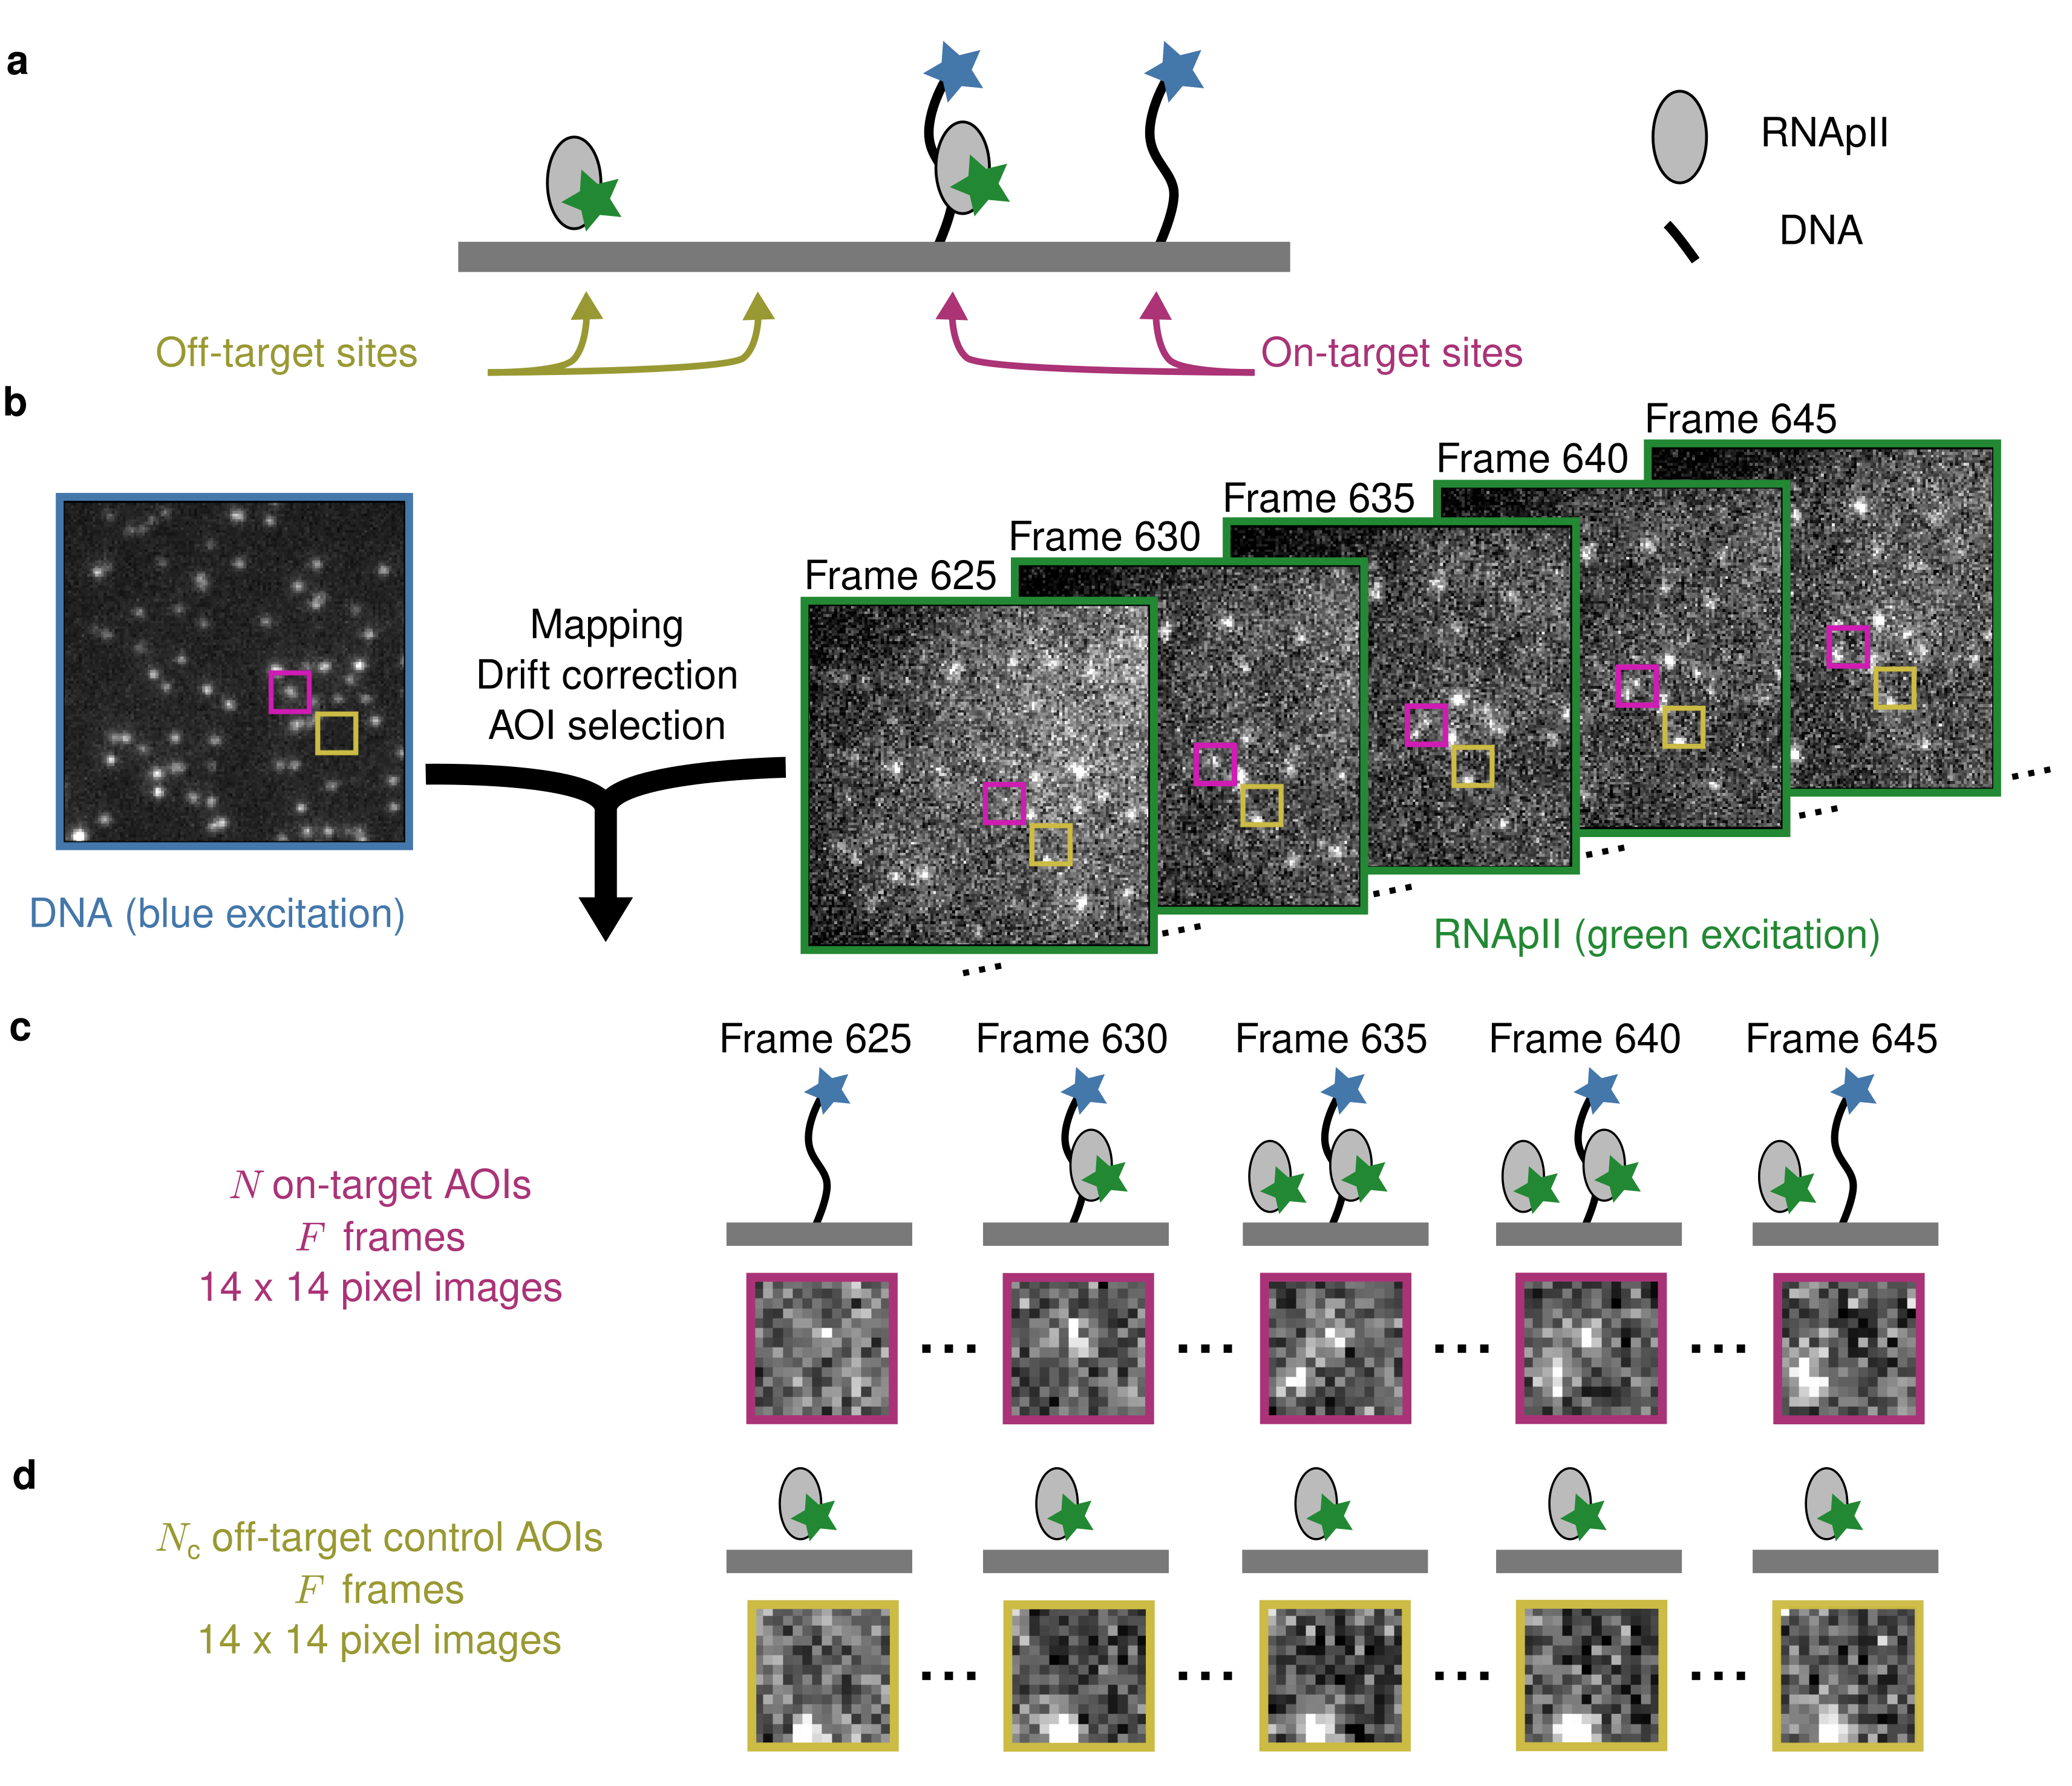
\includegraphics[width=\textwidth]{figures/figure1/figure1.png}
\caption{\textbf{Example CoSMoS experiment.} \textbf{a}, Experiment schematic. DNA target molecules labeled with a blue-excited fluorescent dye (blue star) are tethered to the microscope slide surface. RNA polymerase II (RNApII) binder molecules labeled with a green-excited dye (green star) are present in solution. \textbf{b}, Data collection and preprocessing. After collecting a single image with blue excitation to identify the location of the DNA molecules, a time sequence of RNApII images were collected with green excitation.  Preprocessing of the images includes localization of target molecules in the blue channel, selection of on-target and off-target areas of interest (AOIs; examples shown in purple and yellow, respectively), registration of target and binder channels, and time-dependent drift correction. \textbf{c}, On-target data. Data are time sequences of $14 \times 14$ pixel AOI images centered at each target molecule. Frames show on-target (e.g., frame 630) and off-target (e.g., frame 645) binding of RNApII molecules. \textbf{d}, Off-target control data. Control data consists of images collected from randomly selected sites at which no target molecule is present. Dataset: polII (See Table S1). }
\label{fig:cosmos_experiment}
\end{figure}


\begin{figure}[t]
\centering
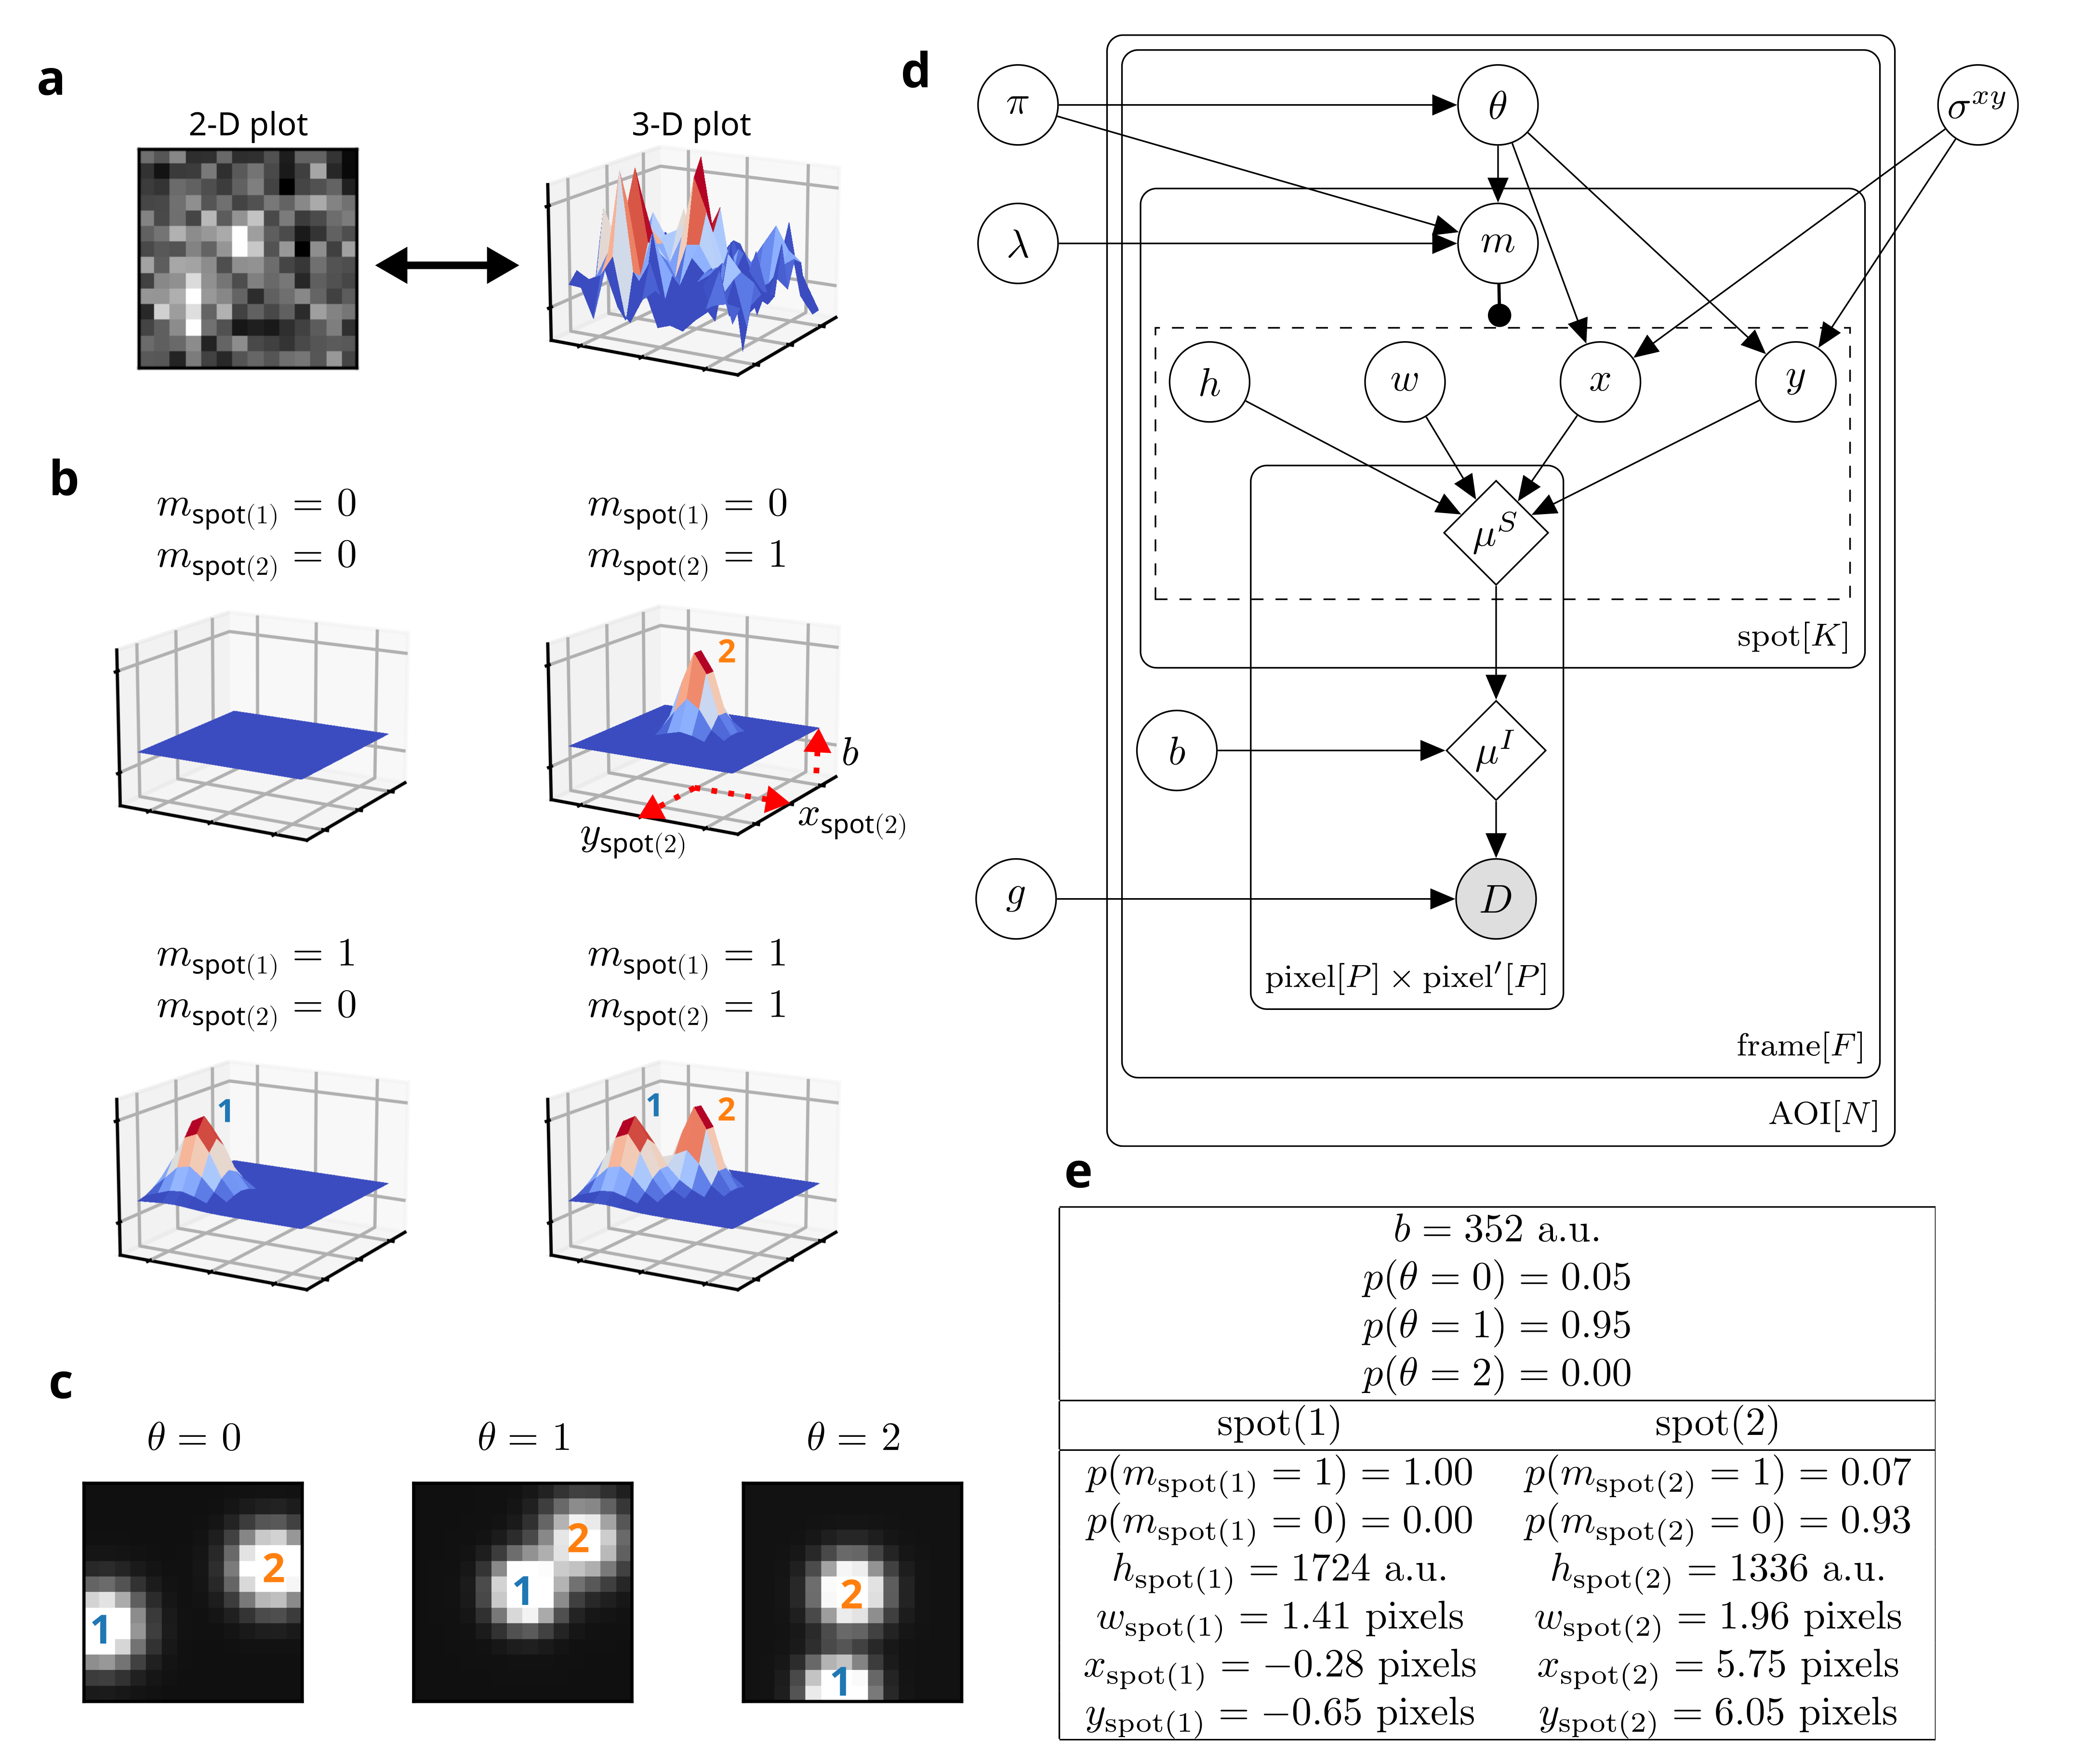
\includegraphics[width=\textwidth]{figures/figure2/figure2.png}
\label{fig:tapqir_model}
\end{figure}

%\addtocounter{figure}{-1}
\begin{figure} [t!]
\caption{\textbf{Depiction of the generative model and model parameters.} \textbf{a}, Example observed data ($D$). The data is a matrix (AOI) of $14 \times 14$ pixel intensities which is here represented as both a 2-D grayscale image and as a 3-D intensity plot. The image contains two spots, one is centered at target location (image center) and the other is located off-target. \textbf{b}, Examples of four idealized noise-free image representations ($\mu^I$). Image representations consist of zero, one, or two idealized spots ($\mu^S$) superimposed on a constant background ($b$). Each fluorescent spot is represented as a 2-D Gaussian parameterized by integrated intensity ($h$), width ($w$), and position ($x$, $y$). We assume that each image contains a maximum of one specifically bound fluorescent molecule. The presence of spots is encoded in the binary spot existence indicator $m$. \textbf{c}, Simulated idealized images illustrating different values of the target-specific index parameter $\theta$. $\theta = 0$ corresponds to a case when no specifically bound molecule is present; $\theta = 1$ or 2 corresponds to the cases in which the specifically bound molecule is spot 1 or 2, respectively. \textbf{d}, Condensed graphical representation of the probabilistic generative model. Model parameters are depicted as circles and deterministic functions as diamonds. Observed image ($D$) is represented by a shaded circle. Related nodes are connected by edges, with an arrow pointing towards the dependent node (e.g., the shape of the 2-D Gaussian spot $\mu^S$ depends on spot parameters $h$, $w$, $x$, and $y$). The dashed box represents activation of spot parameters based on the spot existence indicator $m$. Plates (rounded rectangles) contain entities that are repeated for the number of instances displayed at the bottom-right corner: number of AOIs ($N$), frame count ($F$), and/or maximum number of spots in a single image ($K=2$). A more complete version of the graphical model specifying the relevant probability distributions is given in Supplementary Figure 2A. \textbf{e}, Table of maximum \emph{a~posteriori} (MAP) parameter values inferred from applying model (\textbf{d}) to the full dataset containing the image in (\textbf{a}). Image models in (\textbf{b}) correspond to parameters shown. }
\end{figure}

\begin{figure}[t]
\centering
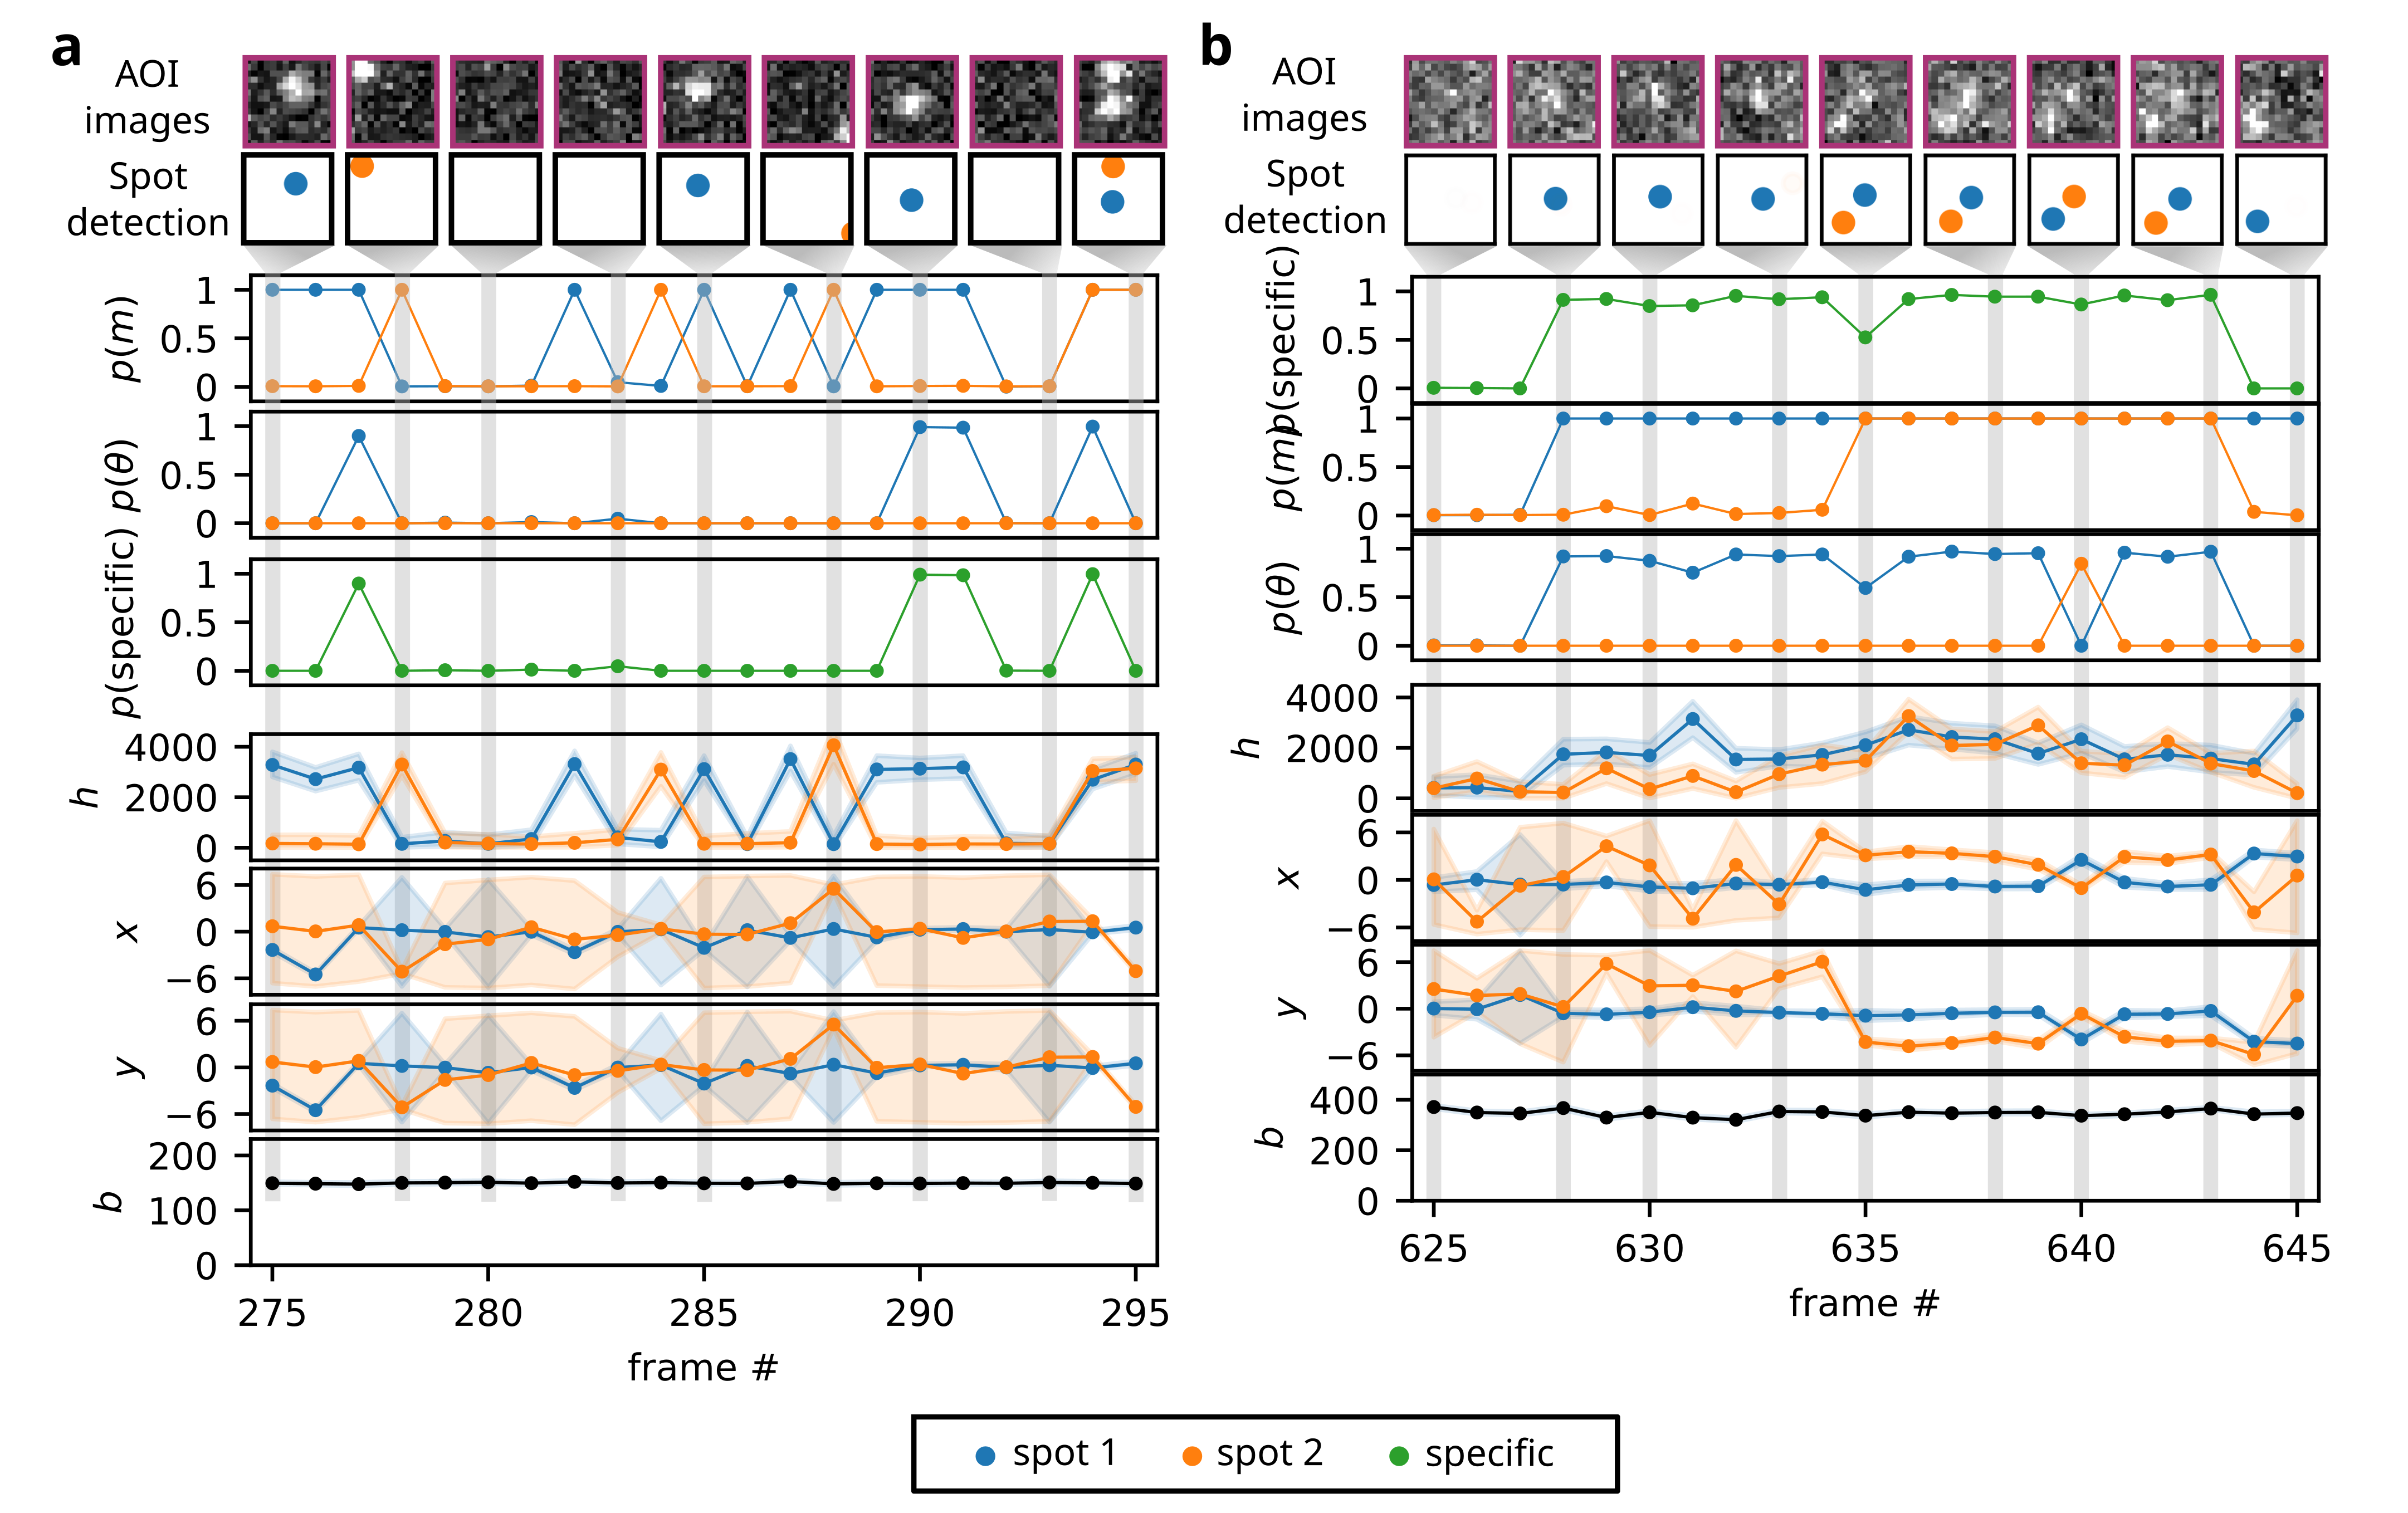
\includegraphics[width=\textwidth]{figures/figure3/figure3.png}
\caption{\textbf{Tapqir analysis and inferred model parameters.} \textbf{a},\textbf{b}, Tapqir was applied to simulated data (\textbf{a}) (height3000 in Supplementary Data 1) and experimental data (\textbf{b}) (polII in Extended Data Table 1). Each panel shows a short extract from a single target location in the dataset. AOI images and corresponding schematics of Tapqir detected spots (color transparency corresponds to spot presence probability) are shown for the subset of frames indicated by gray shaded stripes in the plots. Top three plots show the probability of spot $k$ being present $p(m_{\mathsf{spot}(k)}=1)$, the probability of spot $k$ being target-specific $p(\theta=k)$, and the probability of there being any target-specific spot in a frame $p(\mathsf{specific}) = p(\theta>0)$.  Bottom four graphs show mean values (points) with estimated uncertainties (shading, $95\%$ CI) for the inferred integrated spot intensity $h$, spot position $x$ and $y$, and background intensity $b$. }
\label{fig:tapqir_analysis}
\end{figure}



\begin{figure}[t]
\centering
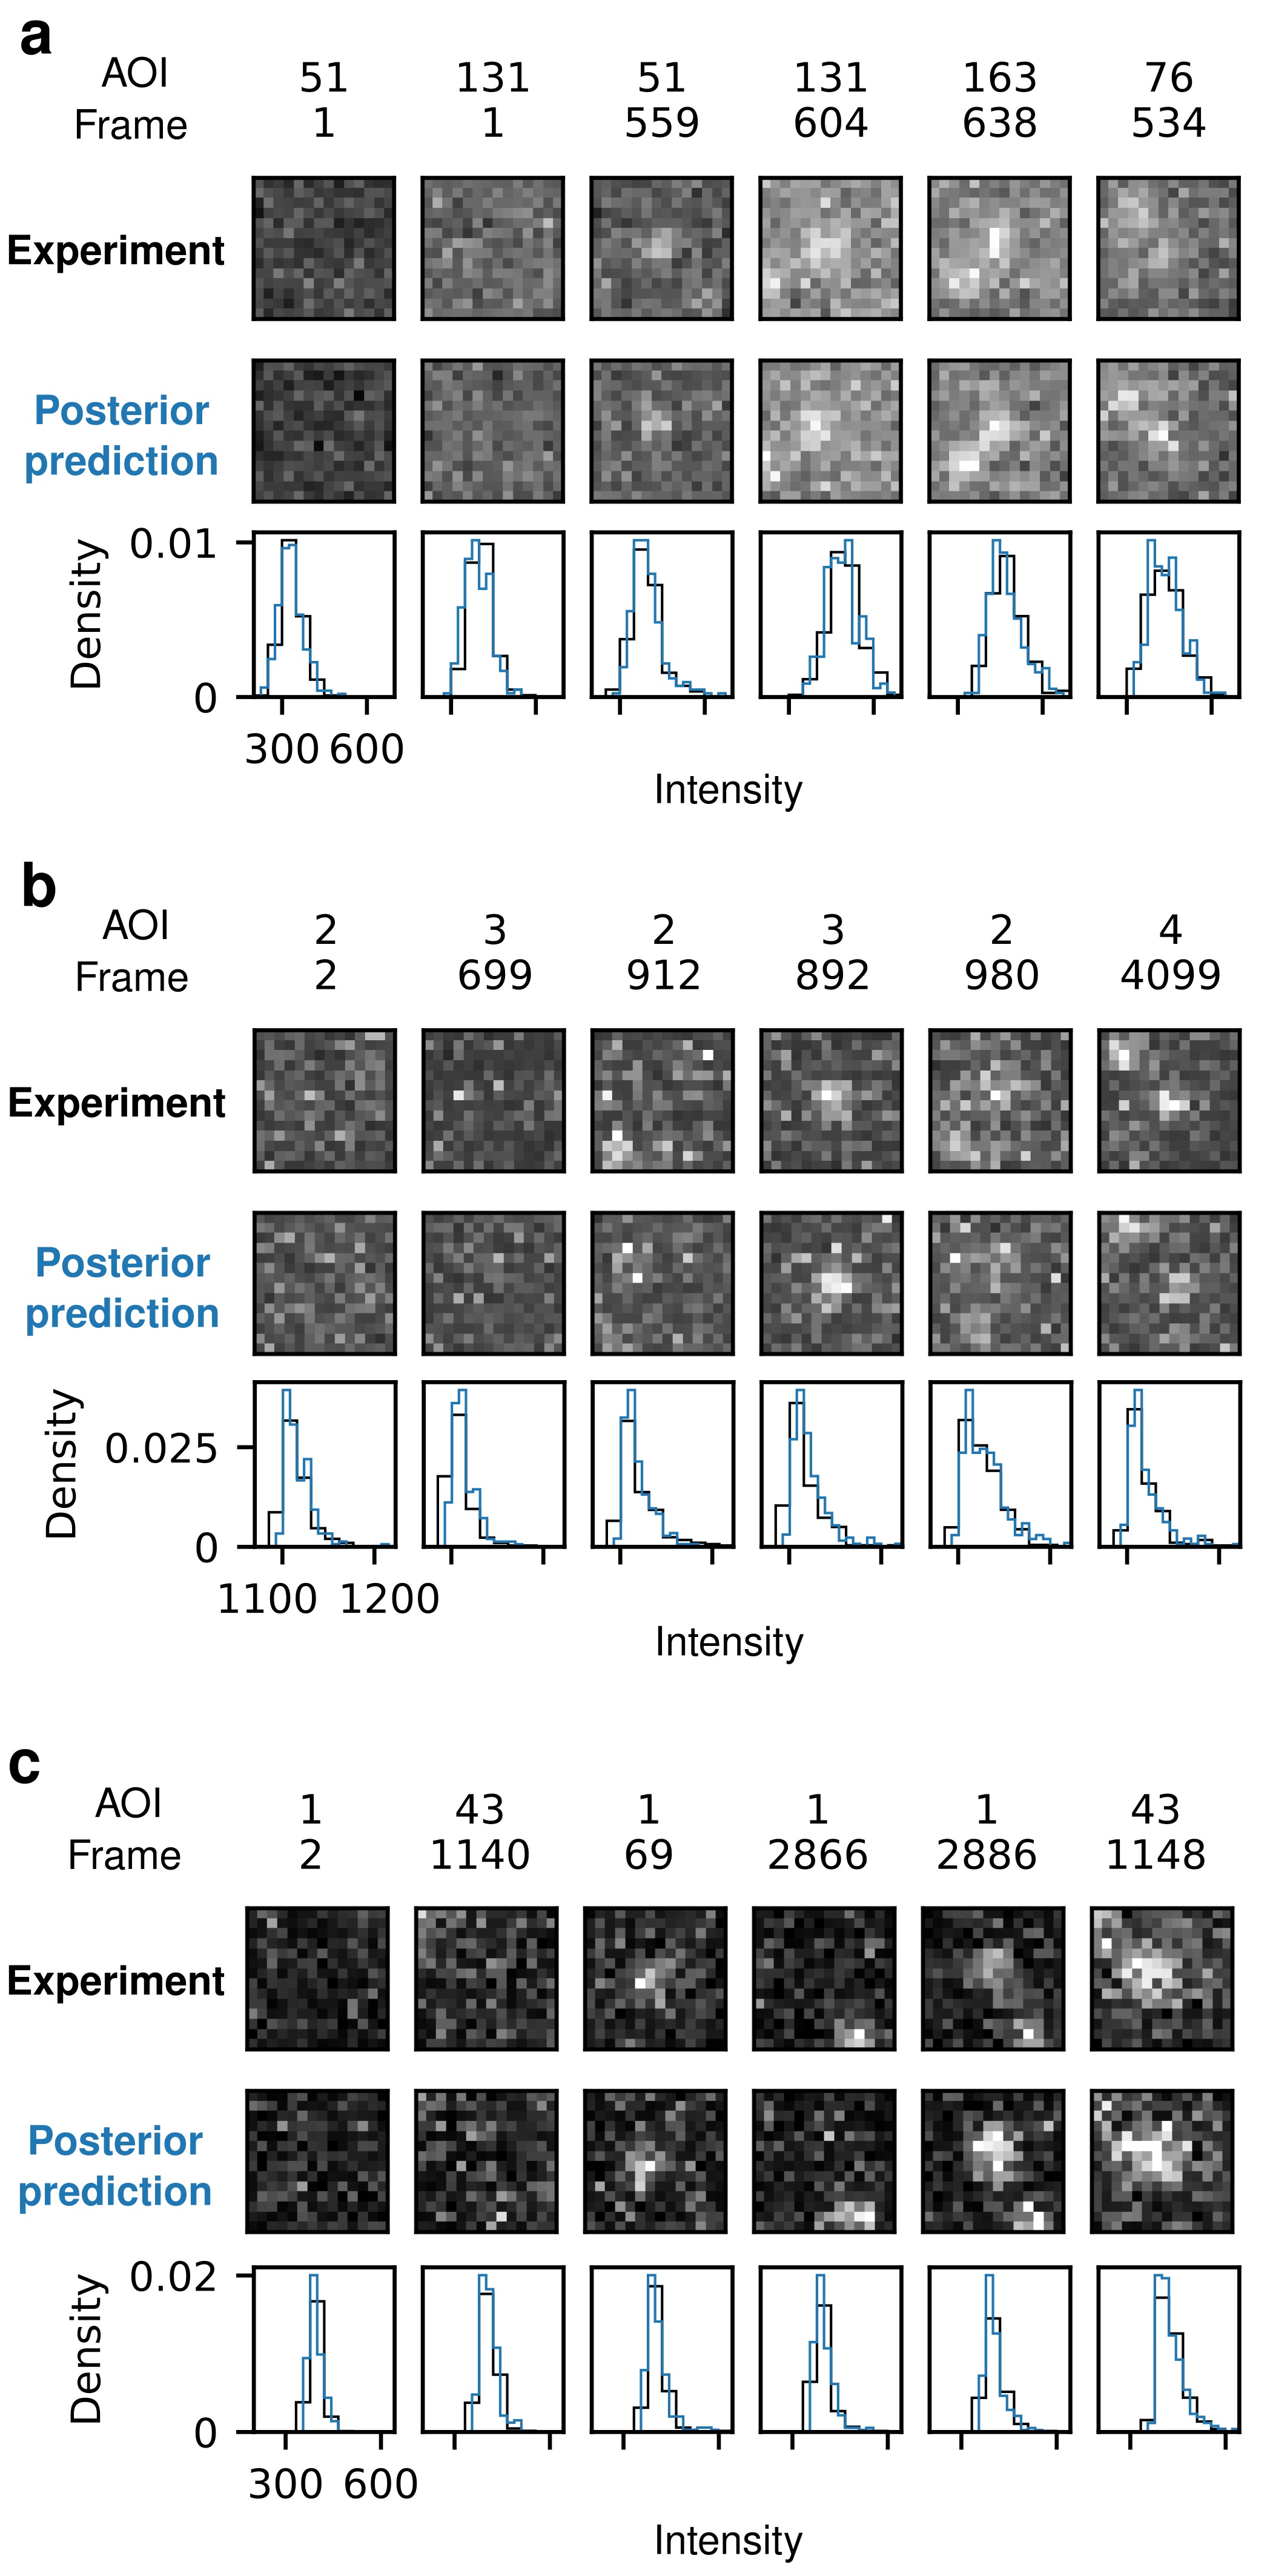
\includegraphics[width=89mm]{figures/figure4/figure4.png}
\caption{\textbf{Reproduction of experimental data by posterior predictive sampling.} Example frames are shown from datasets polII (\textbf{a}: $\mathrm{SNR}=1.61$), NusG (\textbf{b}: $\mathrm{SNR}=4.37$), and $\sigma^{54}$ (\textbf{c}: $\mathrm{SNR}=3.87$) (Extended Data Table 1). In each panel top row shows images of the experimental data and middle row shows images sampled from the posterior distributions. Bottom row shows intensity distributions of experimental data and posterior predictions of images shown. }
\label{fig:posterior_samples}
\end{figure}

\begin{figure}[t]
\centering
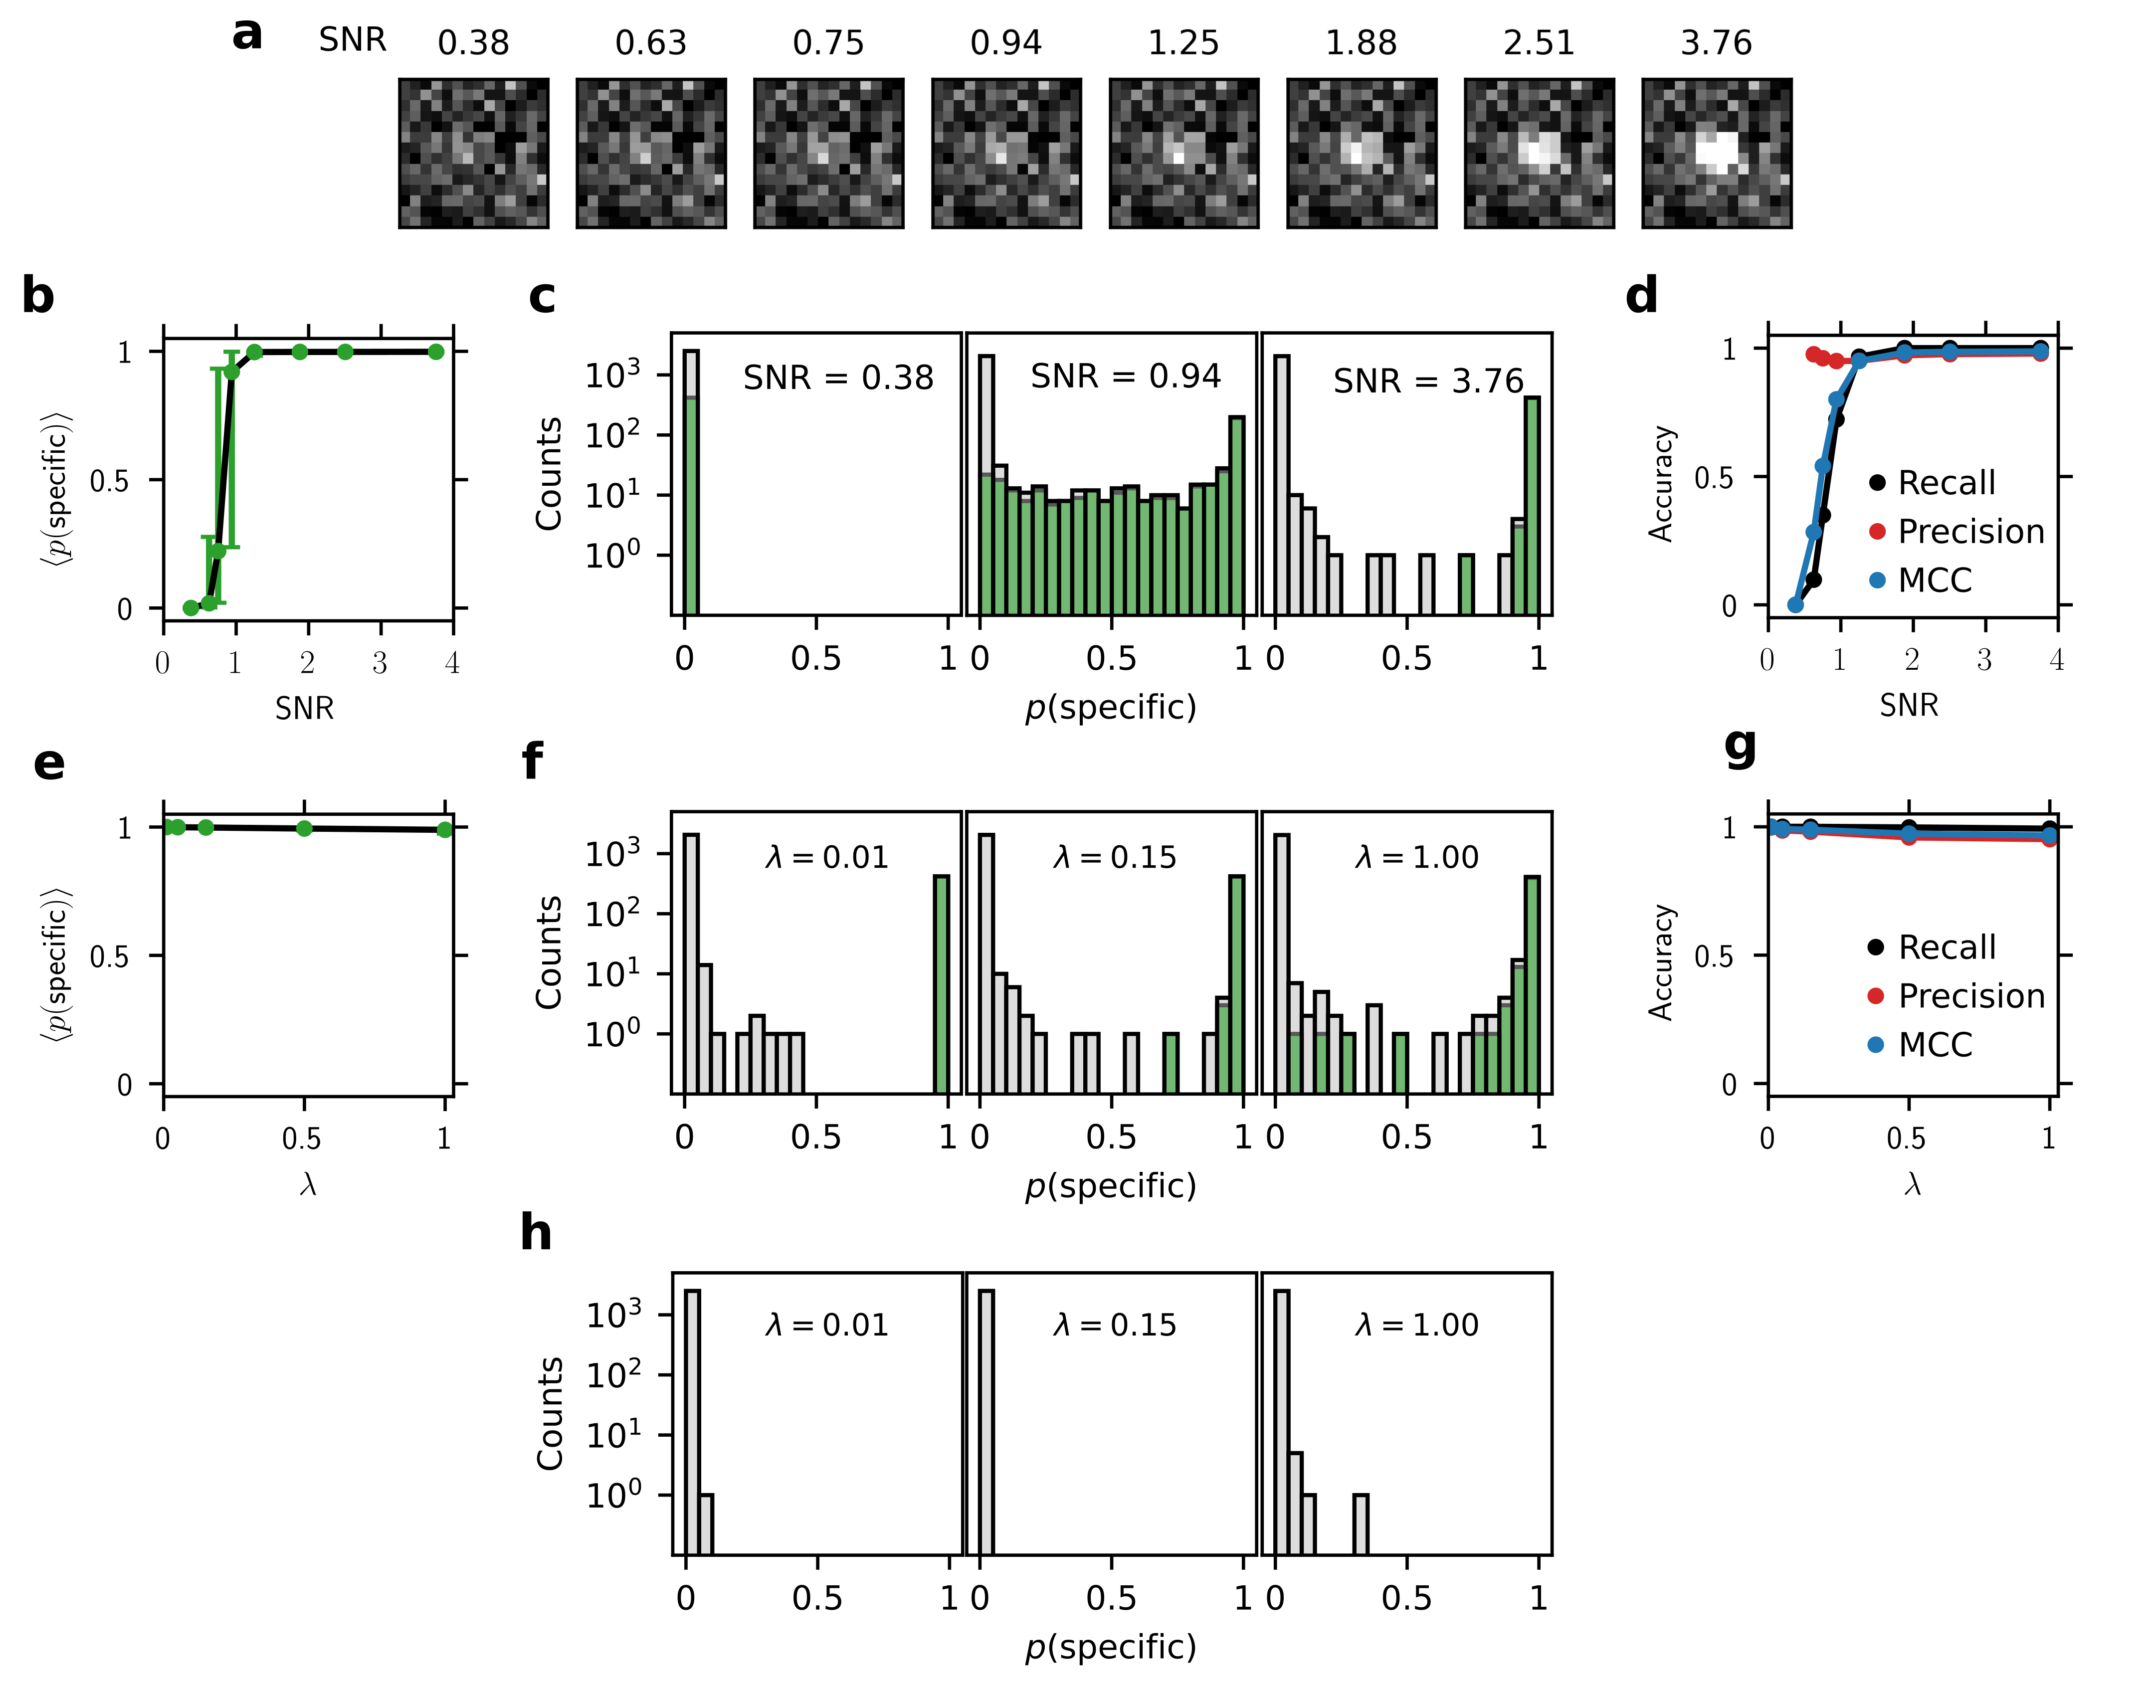
\includegraphics[width=1\textwidth]{figures/figure5/figure5.png}
\caption{\textbf{Tapqir performance on simulated data with different SNRs or different non-specific binding rates.} \textbf{a-d}, Analysis of the simulated data over a range of SNR where SNR was varied by changing spot intensity  $h$ while keeping other parameters constant (Supplementary Data 1). \textbf{a}, Example images showing the appearance of the same target-specific spot simulated with increasing SNR.   \textbf{b}, Mean of Tapqir-calculated target-specific spot probability $p(\mathsf{specific})$ (with 68\% C.I.) for the subset of images where target-specific spots  are known to be present. \textbf{c}, Histograms of $p(\mathsf{specific})$ for selected simulations with SNR indicated. Data are shown as stacked bars for images known to have (green, 15\%) or not have (gray, 85\%) target-specific spots.  Count is zero for bins where bars are not shown. \textbf{d}, Accuracy of Tapqir image classification with respect to presence/absence of a target-specific spot. Accuracy was assessed by MCC, recall, and precision (see Text and Methods). \textbf{e-g}, Same as in (\textbf{b-d}) but for the data simulated over a range of non-specific binding rates $\lambda$ at fixed SNR = 3.76 (Supplementary Data 3). \textbf{h}, Same as in (\textbf{c}) but for the data simulated over a range of non-specific binding rates $\lambda$ with no target-specific binding ($\pi = 0$) (Supplementary Data 4).}
\label{fig:tapqir_performance}
\end{figure}

% figure 6
\begin{figure}[t]
\centering
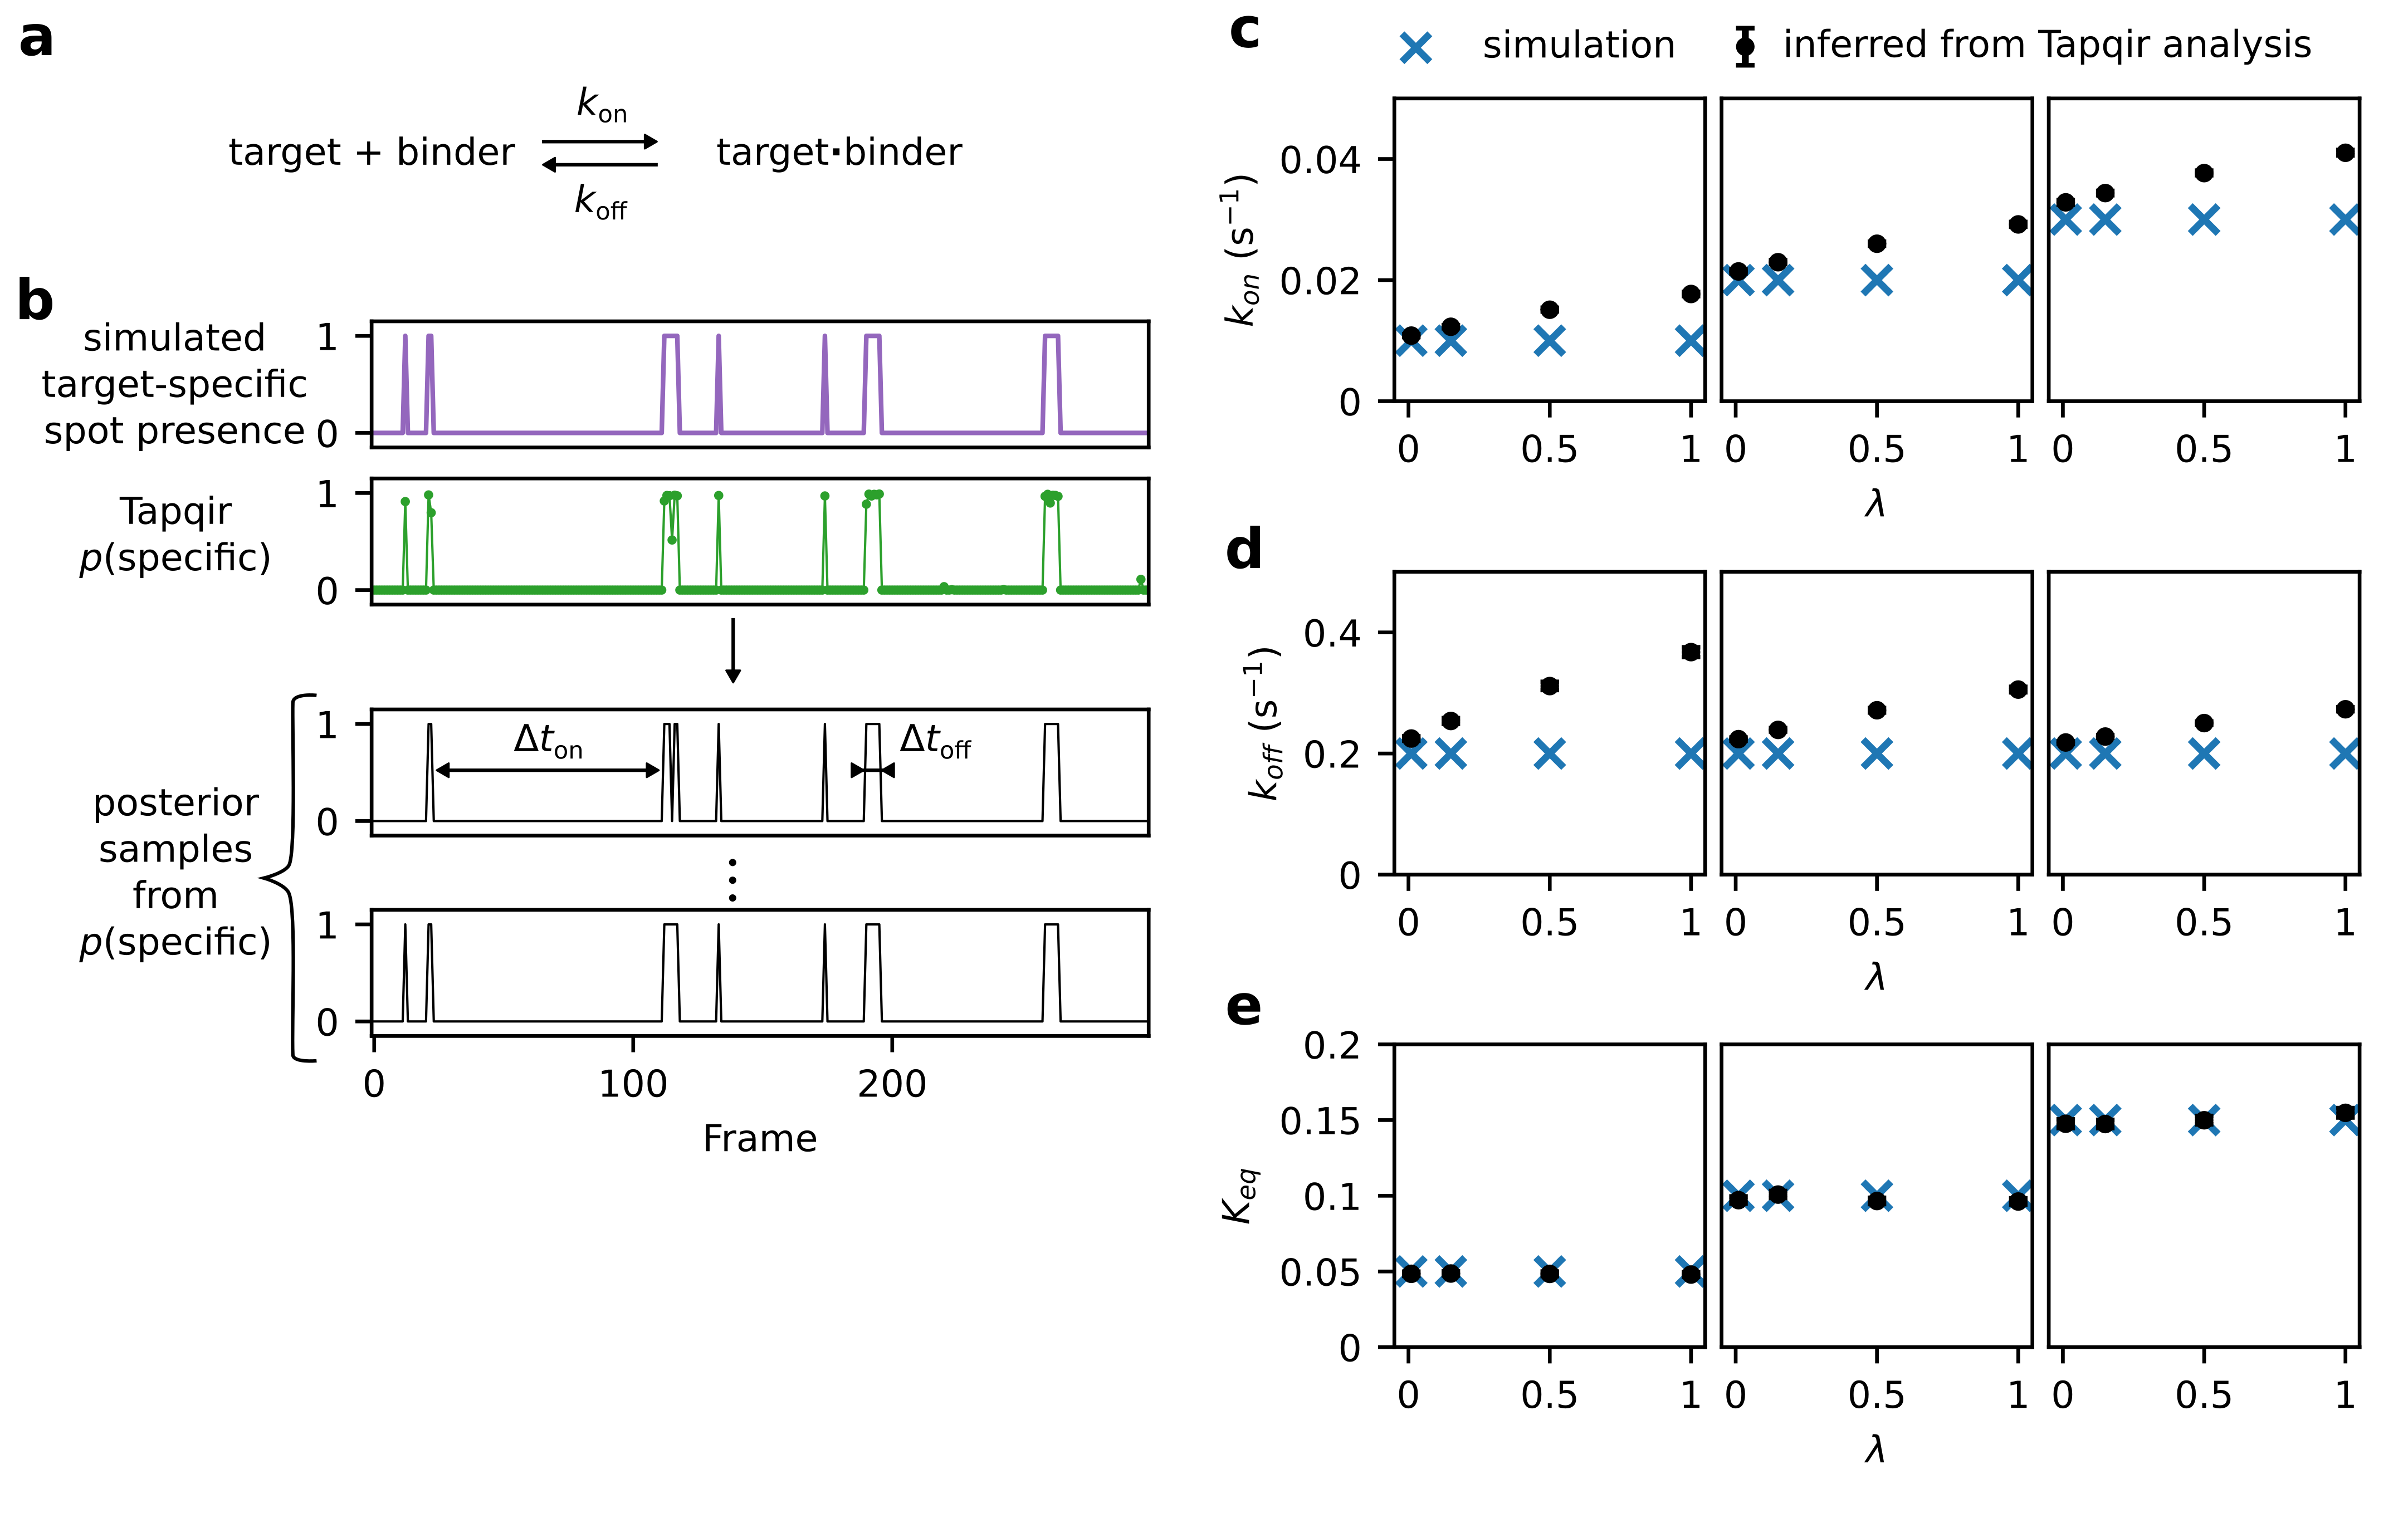
\includegraphics[width=130mm]{figures/figure6/figure6.png}
\caption{\textbf{Tapqir analysis of association/dissociation kinetics and thermodynamics.} \textbf{a} Chemical reaction scheme for a one-step association/dissociation reaction at equilibrium with apparent first-order binding and dissociation rate constants $k_{\mathrm{on}}$ and $k_{\mathrm{off}}$, respectively. \textbf{b}, Simulation of the reaction in (\textbf{a}) and scheme for analysis with Tapqir. Simulation used $\mathrm{SNR} = 3.76$, $k_\mathrm{on} = 0.02$ s$^{-1}$, $k_\mathrm{off} = 0.2$ s$^{-1}$, and a high target-nonspecific binding frequency $\lambda = 1$ (Supplementary Data X, dataset kon0.02lambda1). Full datasets consisted of 100 AOI locations and 1000 frames for both on-target and control data. Shown is a short extract of data from a single target location in the simulation.  Plots show simulated presence/absence of the target-specific spot  (purple) and Tapqir-calculated estimate of corresponding target-specific spot probability $p(\mathsf{specific})$ (green). One thousand binary traces (black) were sampled from the $p(\mathsf{specific})$ posterior distribution and used to compute binding-present ($\Delta t_\mathrm{on}$) and binding-absent ($\Delta t_\mathrm{off}$) dwell times. \textbf{c,d,e}, Kinetic and equilibrium constants from a set of simulations using a range of $k_\mathrm{on}$ values and  target-nonspecific spot frequencies $\lambda$, with constant $k_\mathrm{off} = 0.2$ s$^{-1}$. \textbf{c} Values of $k_{\mathrm{on}}$ used in simulation (blue) and inferred from the distribution of $\Delta t_\mathrm{off}$ (black). \textbf{d}, Same as (\textbf{c}) but for $k_{\mathrm{off}}$ used in simulation and inferred from $\Delta t_\mathrm{on}$. \textbf{e},  Same as (\textbf{c}) but for dissociation equilibrium constant $K_{\mathrm{eq}} = k_{\mathrm{on}} / k_{\mathrm{off}}$ used in simulation and inferred from $\pi$ as $K_{\mathrm{eq}} = \pi / (1 - \pi)$. }
\label{fig:kinetic_analysis}
\end{figure}

% figure 7
\begin{figure}[t]
\centering
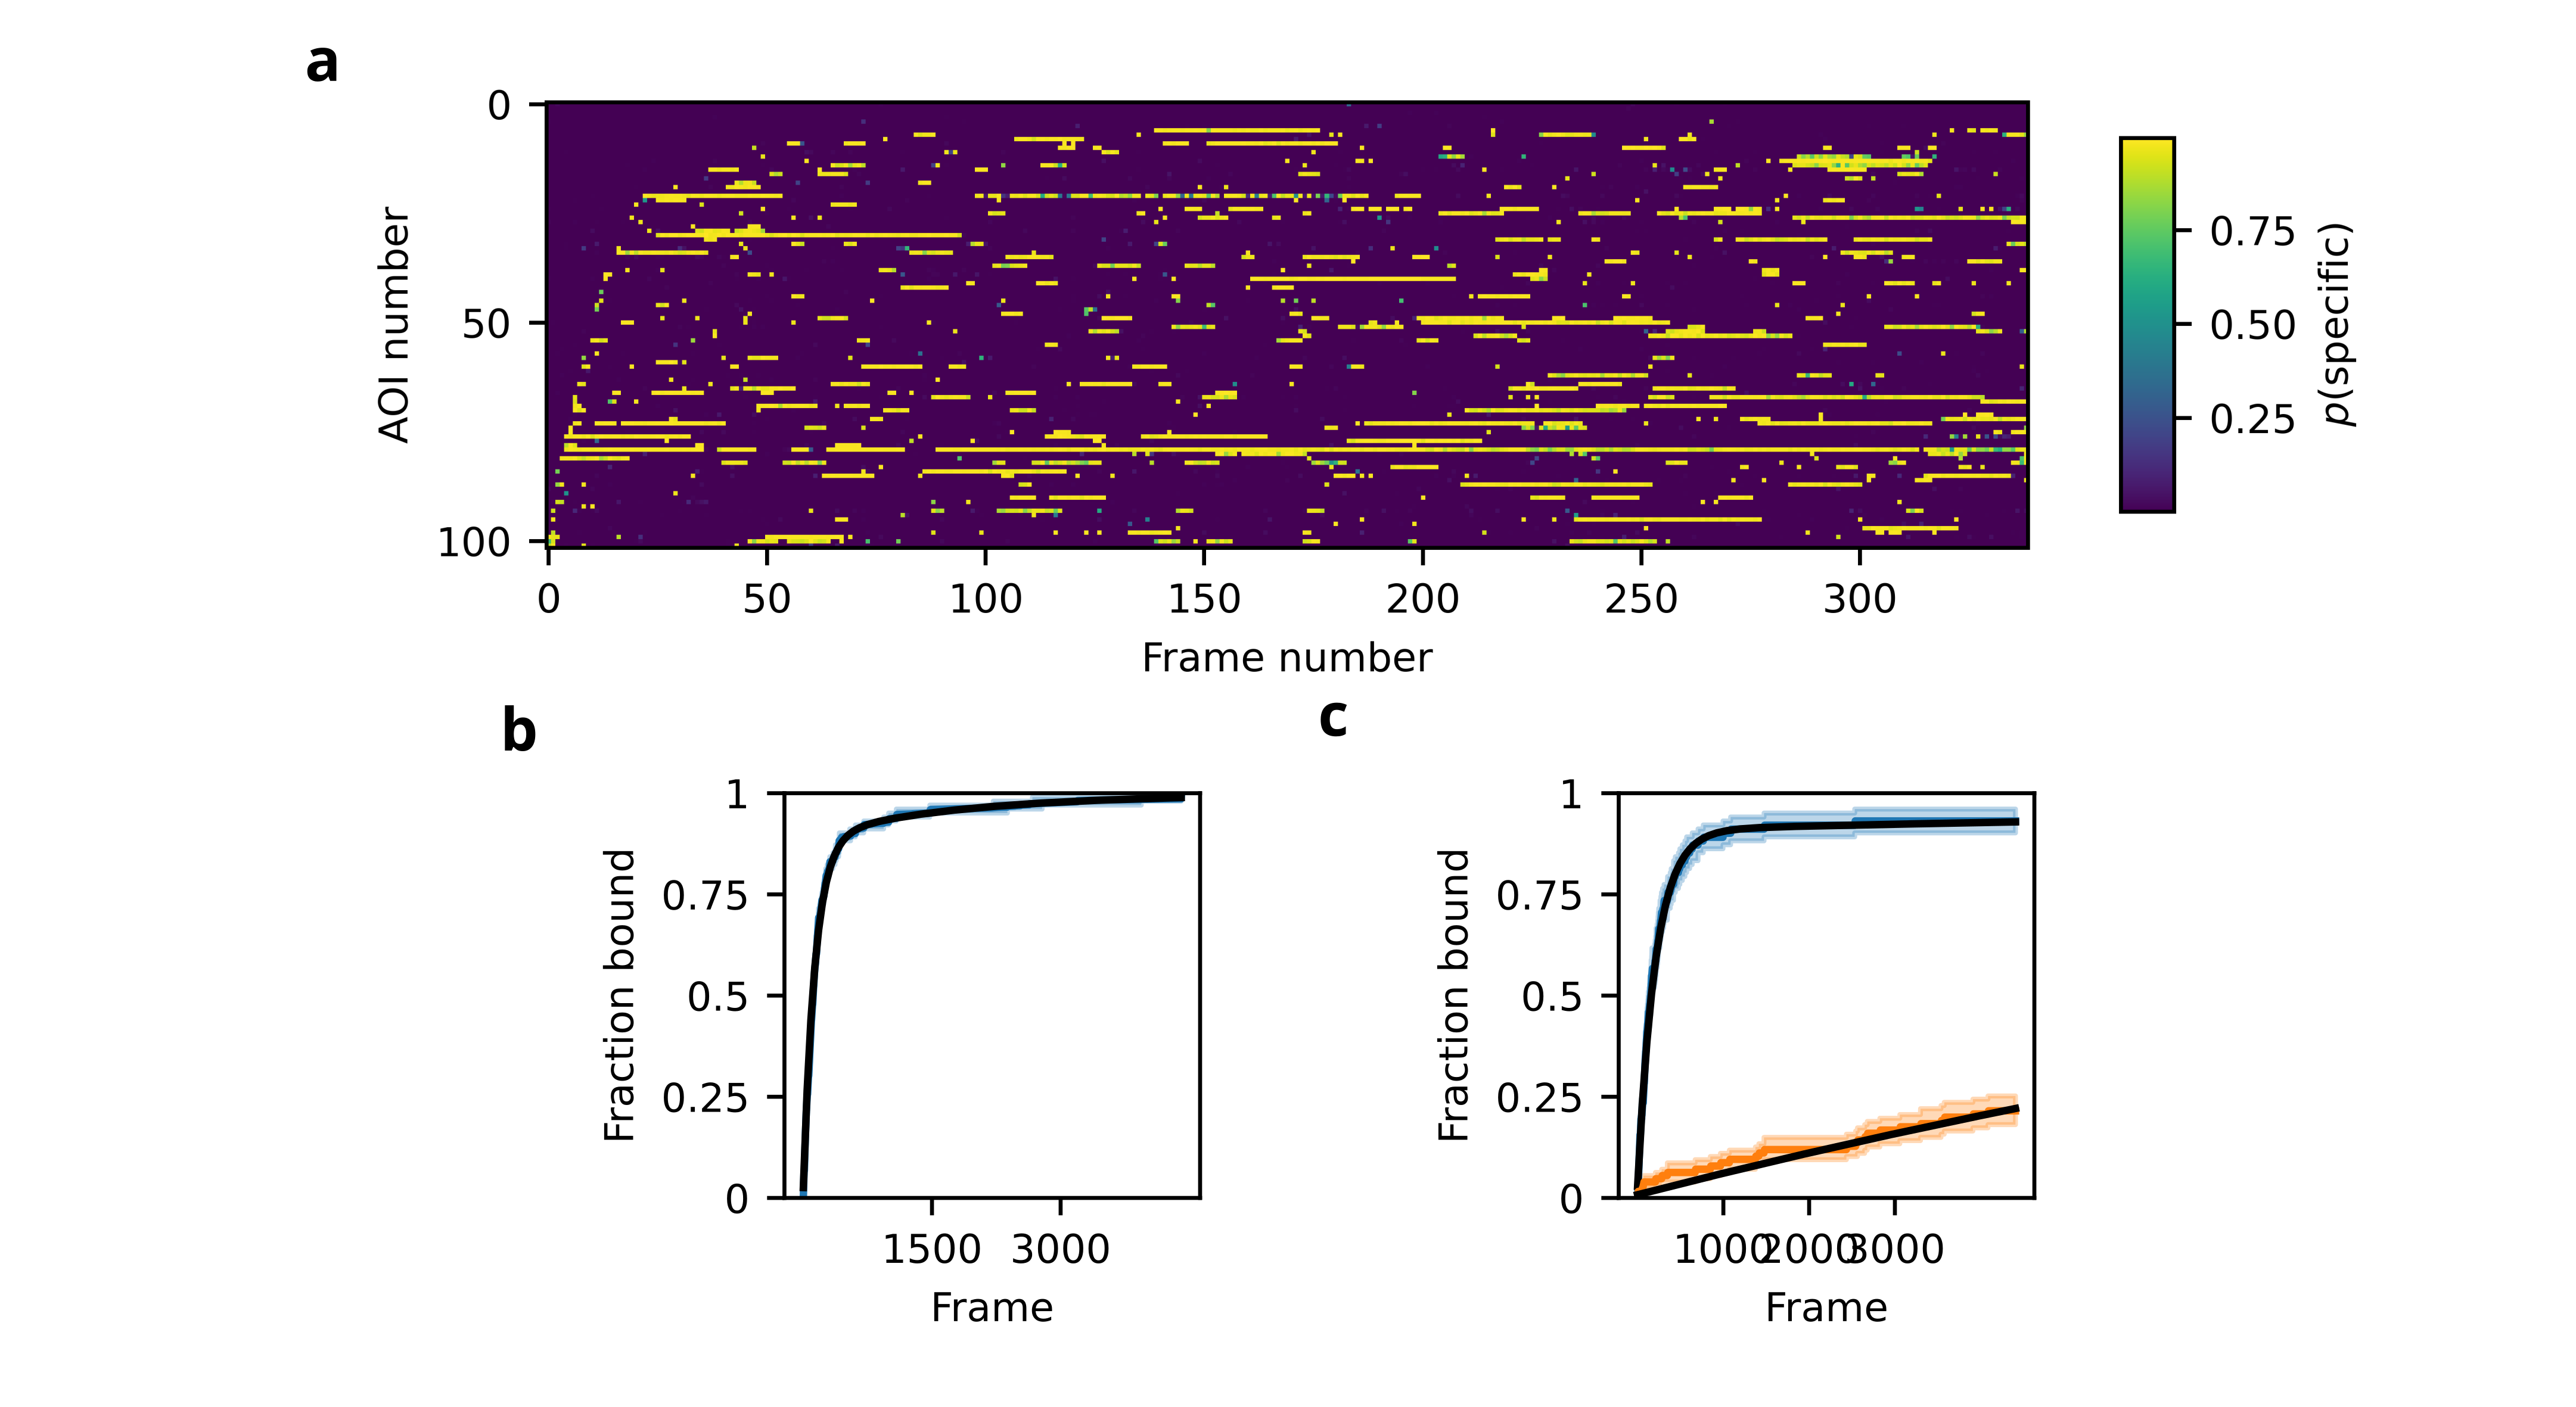
\includegraphics[width=183mm]{figures/figure7/figure7.png}
\caption{\textbf{Kinetic analysis of experimental data.}   \textbf{a}, Rastergram representation of Tapqir-calculated target-specific spot  probabilities $p(\mathsf{specific})$ (color scale) for every 8$^th$ frame of data at 102 different target locations.  AOIs were ordered by decreasing times-to-first-binding. Data set: $\sigma^{54}$ in Table S1. \textbf{b,c}, Determining the association rate constant for the same data set by  time-to-first-binding analysis using Tapqir (\textbf{b}) and an empirical spot-picker method (\textbf{c}) (ref).   Cumulative fraction of target sites that exhibited one or more binding events by the indicated time (blue) and fit curve (black) yielding best-fit values for $k_\mathrm{a}$, $k_\mathrm{ns}$, and $A_\mathrm{f}$. Fitting protocol is different for the two methods; the spot-picker method fits both the target sites and off-target control data (orange) whereas Tapqir incorporates the control data in its $p(\mathsf{specific})$ calculation.
}
\label{fig:experimental_data}
\end{figure}